%!TEX root=../robocert.tex
\begin{figure}[htb]
	\centering
	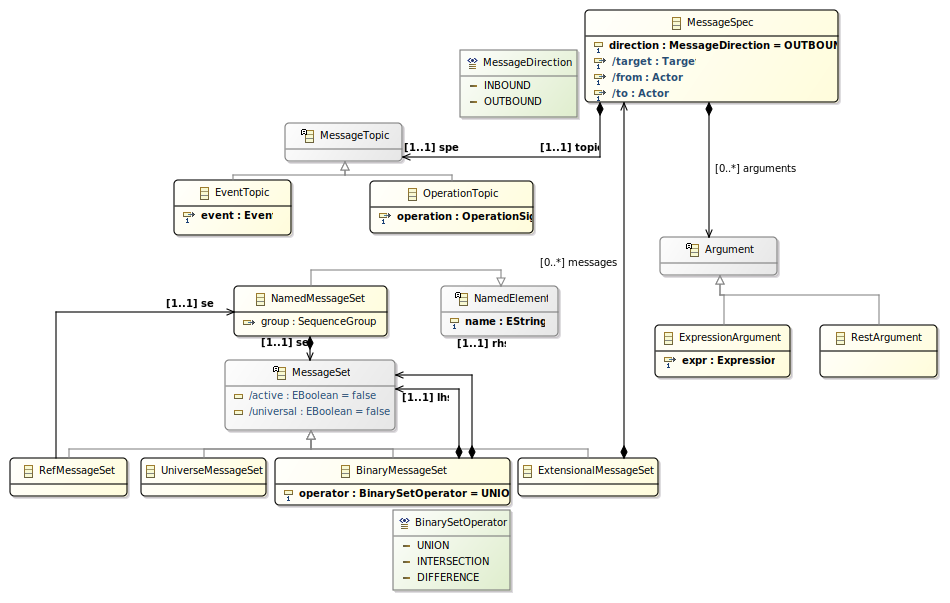
\includegraphics[width=\textwidth]{diagrams/Messages}
	\caption{Class diagram for the part of the \langname{} metamodel dealing with messages.}
	\label{fig:metamodel-messages}
\end{figure}

\noindent
Messages are introduced into a sequence diagram
in \mmessageset s and \marrowaction s.  They capture the various forms of
communication in \robochart: events, operations, and \todo{eventually}
variables.

\Cref{fig:metamodel-messages} depicts the part of the metamodel concerning
messages between actors.

\subsection{\mmessageset}\label{ssec:metamodel-messages-sets}

A \mmessageset{} expresses a set of messages allowed 
inside a \msequencegap.  There are four types of \mmessageset:

\begin{itemize}
\item
  a \muniversemessageset{} represents the universal set containing 
  all possible messages;
\item	
  an \mextensionalmessageset{} is a set (expressed as an unordered list) of
  zero or more \mgapmessagespec s, themselves
  a type of \mmessagespec{} (\cref{sec:metamodel-messages});
\item
  a \mrefmessageset{} refers to a \mnamedmessageset{} attached to the
  sequence group;
\item
  a \mbinarymessageset{} is a binary operator over two other \mmessageset s
  (operators are union, intersection, and difference).
\end{itemize}

There is not yet any meaningful extra data stored in
\mgapmessagespec s that is not present in \mmessagespec s, but this is subject
to change.

\begin{lstlisting}[style=Example]
universe                  // UniverseMessageSet
{| ->op O1(), ->op O2 |}  // ExtensionalMessageSet
->op O1()                 // singleton ExtensionalMessageSet
set S                     // RefMessageSet
set X or set Y            // UNION BinaryMessageSet
set X and set Y           // INTER BinaryMessageSet
set X except set Y        // DIFF BinaryMessageSet
\end{lstlisting}

\subsection{\mnamedmessageset}\label{ssec:metamodel-messages-named-sets}

A \mnamedmessageset{} attaches a name to a \mmessageset, so that it can be reused
inside a \msequence.

\begin{lstlisting}[style=Example]
message set S: {| ->op O1(), ->op O2 |}
\end{lstlisting}

\subsection{\mmessagespec}

A \mmessagespec{} is a specification on the types of communication that can
happen before or during an action.  Each \mmessagespec{} contains:

\begin{itemize}
\item
  a \mmessagedirection; \emph{outbound} from \mtarget{} to \mworld,
  or \emph{inbound} from \mworld{} to \mtarget;
\item
  the \mmessagetopic{} (\cref{ssec:metamodel-messages-topics}) specifying
  the type of communication that the spec is capturing.
\end{itemize}

It is possible to infer the \mtarget{} and \mworld{} related by a
\mmessagespec{} through its containing \msequencegroup.  From these
and the \mmessagedirection, we can further infer the source (`from')
and destination (`to') \mactor s.  The target, from, and to actors are
available in EMF as derived references.

\begin{figure}[H]

\begin{subfigure}[t]{\egtextwidth}
\begin{lstlisting}[style=Example]
->op O1()
// outbound MessageSpec with OperationTopic

<-event E
// inbound MessageSpec with EventTopic
\end{lstlisting}
\end{subfigure}
\hfill
\begin{subfigure}[t]{\eggraphicalwidth}
\gsecaption
\centering
\begin{tikzpicture}
\matrix[diagram]{
    \node[rcmodule](mstart) {\egtarget}; & \node[world](wstart) {\egworld}; \\
	\coordinate(mo); & \coordinate(wo); \\
	\coordinate(me); & \coordinate(we); \\
	\coordinate(mend); & \coordinate(wend); \\
};
\draw[lifeline] (wstart) -- (wo) -- (we) -- (wend);
\draw[lifeline] (mstart) -- (mo) -- (me) -- (mend);
\draw (mo) edge[oarrow, "O1()"] (wo);
\draw (we) edge[earrow, "E"'] (me);
\end{tikzpicture}
\end{subfigure}

\end{figure}

\subsection{\mmessagetopic}\label{ssec:metamodel-messages-topics}

A \mmessagetopic{} identifies the type of communication in a
\mmessagespec{}.  There are two types of topic, corresponding to
\robochart{} operations (\moperationtopic) and events (\meventtopic)
\todo{variable topics will arrive later on; \ghissue{24}}.
Each contains a reference to the signature of the respective construct.

\begin{lstlisting}[style=Example]
op O1()  // OperationTopic
event E  // EventTopic
\end{lstlisting}

\subsection{\margument}\label{ssec:metamodel-messages-arguments}

An \margument{} is a pattern that specifies (and possibly binds) one or more
arguments in
a message.  There are two types of argument:

\begin{itemize}
\item
  \mexpressionargument, which specifies that the argument is equal to the
  value of a particular \robochart{} expression;
  \todo{the \langname{} CSP generator doesn't yet properly protect against this being
    an expression not expressible as a prefix}
\item
  \mrestargument, which matches \emph{all} following arguments and permits
  them to be any value.
  \todo{This mainly exists because it's very easy to specify in CSP.  Ideally
    we'll have something that allows wildcards on arbitrary parameters, in
    which case this might be confusing to have also.}
\end{itemize}

\begin{lstlisting}[style=Example]
42  // ExpressionArgument containing integer literal
... // RestArgument
\end{lstlisting}

%%% Local Variables:
%%% mode: latex
%%% TeX-master: "../robocert"
%%% End:
